\documentclass[crop=false]{standalone}
\usepackage{standard}

\begin{document}
  \section{Vorbereitung} % (fold)
  \label{sub:Vorbereitung}

    \subsection{Einlesen der Szenendaten} % (fold)
    \label{ssub:einlesen_der_daten}
      \paragraph{STL-Dateiformat}
      Das STL-Dateiformat (engl.: \textit{stereolithography}) beschreibt die Oberfläche von 3D-Körpern mit Hilfe von Dreiecksfacetten.
      Jede Dreiecksfacette wird durch die drei Eckpunkte und die zugehörige Flächennormale des Dreieckes charakterisiert.
      Bei der hier verwendeten Variante handelt es sich um die binäre Form des Dateiformats, da so eine erhebliche Reduktion der Dateigröße erreicht wird.
      Zudem übersteigt die Einlesegeschwindigkeit des binären Formats die des Standardformats um mehrere Größenordnungen.

      Das Einlesen einer STL-Datei wird im C++-Code durch die Klasse \texttt{std::fstream} realisiert.
      Diese Klasse ist in jedem C++-Compiler vorhanden, wie es im Sprachstandard festgelegt ist.
      Zunächst wird durch das Auslesen des Dateikopfes die Anzahl der Dreiecke bestimmt.
      Basierend auf dieser Zahl wird ein Array im Arbeitsspeicher alloziert.
      Mithilfe einer \texttt{for}-Schleife werden dann die Daten jedes einzelnen Dreiecks ausgelesen und im Array gespeichert.
      Im Folgenden ist dieses Verfahren durch ein Codebeispiel gezeigt.

      \inputCodeBlock[title = STL Loader]{code/stl_reader.cc}

      \paragraph{OBJ-Dateiformat}
      OBJ (auch \textit{Wavefront OBJ}) ist ein offenes Dateiformat zum Speichern von dreidimensionalen geometrischen Formen.
      Das Format wird von vielen Grafikprogrammen unterstützt und ist daher geeignet für die programm- und plattformübergreifende Weitergabe von 3D-Modellen.
      Es handelt sich um ein ASCII-basiertes Dateiformat, welches zeilenweise ausgelesen werden muss.
      Jede Zeile enthält einen Befehl mit den entsprechenden Argumenten.
      Für dieses Projekt wurden nur drei der vielen Befehle verwendet.

      \inputCodeBlock[title = OBJ Kommandos,language=]{code/obj_commands.obj}

      Auch bei diesem Dateiformat wurde die Klasse \texttt{std::fstream} verwendet.
      Für die Eckpunkte, die Normalen und die Flächen wurde jeweils ein eigener Container generiert.
      Bei dem Container handelt es sich um das Template \texttt{std::vector} der C++-Standardbibliothek.
      Durch die Verwendung dieses Templates wird das Hinzufügen eingelesener Daten auch bei Überschreitung des reservierten Speichers effizient durchgeführt.
      Alle Koordinaten wurden mit einfacher Genauigkeit in dem Gleitkommatyp \texttt{float} und alle Referenzen auf Eckpunkte oder Normalen im Ganzzahltyp \texttt{int} gespeichert.
    % subsection einlesen_der_daten (end)

    \subsection{Grafische Ausgabe} % (fold)
    \label{ssub:ausgabe}
      Für die graphische Ausgabe wurde die Bibliothek OpenGL zusammen mit dem Framework GLUT verwendet.
      GLUT erstellt einen OpenGL-Context und dient auch als Window-Manager.
      OpenGL wird benötigt um den Pixelpuffer eines Fensters (Array, indem der Status jedes Pixels eines Fensters gespeichert ist) auf dem Bildschirm auszugeben.

      Um sowohl das Einlesen der Dateiformate als auch die Korrektheit des Raytracers zu testen, wurde die Graphics-Engine von OpenGL genutzt.
      Anhand einiger Standardmodelle, wie dem \textit{Conference Room} in Abbildung \ref{fig:raytracer-example}, konnte die korrekte Funktion der Datei-Loader und der graphischen Ausgabe sichergestellt werden.
      \begin{figure}
        \center
        \begin{subfigure}[b]{0.49\textwidth}
          \center
          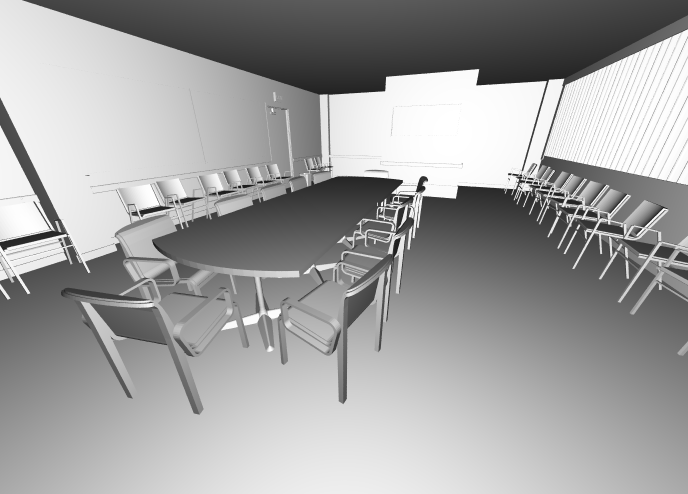
\includegraphics[width=0.95\textwidth]{images/ray_tracer_example.png}
        \end{subfigure}
        \begin{subfigure}[b]{0.49\textwidth}
          \center
          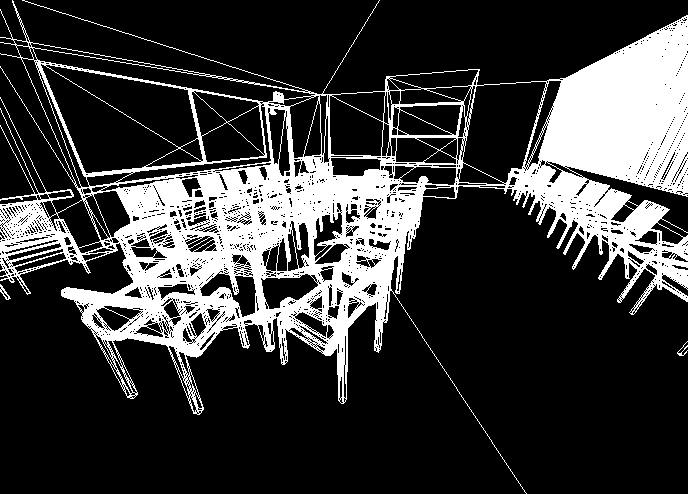
\includegraphics[width=0.95\textwidth]{images/opengl_example.png}
        \end{subfigure}
        \caption{%
          Die Abbildung zeigt die Szene \textit{Conference Room}.
          Auf der linken Seite wurde das Bild mithilfe des Raytracers generiert.
          Die rechte Seite zeigt das \textit{Wireframe} gerendert durch OpenGL.
        }
        \label{fig:raytracer-example}
      \end{figure}
    % subsection ausgabe (end)

    \subsection{Performance-Analyse} % (fold)
    \label{ssub:performance_analyse}
      Damit die Effizienz der Algorithmen objektiv miteinander verglichen werden konnte, wurde die mittlere Zeitspanne zum Erstellen eines Bildes (engl.: \textit{Frame}) für jeden Algorithmus gemessen.
      Das Reziproke dieser Messgröße wird in der Literatur auch als \textit{frames per second} (FPS) bezeichnet.
      Hierfür wurde innerhalb einer festgelegten Zeitspanne (in der Regel 5 Sekunden) gemessen, wie oft der Pixelpuffer neu berechnet und ausgegeben wurde.
      Der Quotient aus der gesamten Zeitspanne und der Anzahl der erzeugten Frames ist dann die mittlere Zeit, die zur Berechnung des Pixelpuffers benötigt wird.

      Die hohe Komplexität der Szenen resultiert in starken Schwankungen der FPS je nach Position und Richtung der Kamera.
      Die verschiedenen Algorithmen arbeiten in unterschiedlichen Raumbereichen mit unterschiedlicher Effizienz.
      Für eine quantitative Analyse dieser Algorithmen wurden aus diesem Grund vorher festgelegte Kamerapfade verwendet.
      Der Beobachter bewegt sich auf diesen Pfaden und misst für jeden gegebenen Punkt die FPS.
      So können die Stärken und Schwächen der einzelnen Algorithmen ermittelt werden.

      Zum Festlegen der Kamerapfade muss eine Szene zunächst von einem Benutzer analysiert werden, um Bereiche mit hohen FPS-Schwankungen zu finden.
      Hierfür wurde die manuelle Steuerung der Kamera durch den Benutzer ermöglicht.
      Zudem existieren auch hochkomplexe Szenen, die nur durch die manuelle Analyse untersucht werden können.
    % subsection performance_analyse (end)
  % section vorarbeit (end)
\end{document}